\part{Exercice 6}

Soit $(\Omega, P)$ un espace probabilisé qui modélise cette situation.

\[
	\forall i \in \{1,2,3\},\,\begin{cases}
		P(A_i) = \frac{1}{3}\\[2mm]
		P_{A_i}(R_i) = 1 - \alpha_i.
	\end{cases}
\]

\begin{enumerate}
	\item Soit $i \in \{1,2,3\}$.
		\begin{align*}
			P_{\overline{R}_i}(A_i) &= \frac{P_{A_i}(\overline{R}_i)\;P(A_i)}{P_{A_i}(\overline{R}_i)\,P(A_i) + P_{\overline{A}_i}(\overline{R}_i)\,P(\overline{A}_i)} \\
			&= \frac{\frac{\alpha_i}{3}}{\frac{\alpha_i}{3} + \frac{2}{3}} \\
			&= \frac{\alpha_i}{2 + \alpha_i} \\
		\end{align*}
	\item Soit $f : x \mapsto \frac{x}{2+x}$ dérivable sur $[0,1]$ et \[
			\forall x \in [0,1],\,f'(x) = \frac{2 + \cancel{x} - \cancel{x}}{(2 + x)^2} > 0
		.\]
		\begin{center}
			\begin{tikzpicture}
				\tkzTabInit{$x$/1,$f$/2}{0,1}
				\tkzTabVar{-/0,+/$\frac{1}{3}$}
			\end{tikzpicture}
		\end{center}
\end{enumerate}

